\chapter{Background}
\label{chap:related_work}


\section{Intrusion Tolerance Overview}

It is unrealistic to make prior assumptions on the attacker's power rather than assuming that he or she is a powerful attacker.
Therefore, researchers and developers have been putting all the efforts on the vulnerability side by trying to reduce the probability of the attacker's success. 
In the following, we make an overview of the different approaches that can be combined to deal with the challenge of providing security and dependability for critical systems.

\subsection*{Prevention}
One of the primary techniques is to try to avoid that vulnerabilities persist in the code throughout all the software development phases until it is in production. 
One way to do that is to detect and remove vulnerabilities during the development and testing stages.
There are three main categories: static, dynamic, and concolic analysis.
A few examples of static analysis are source code verification and validation. 
However, the most common techniques typically over-simplify the protocols to make them formally verifiable. 
Moreover, this process consumes much time, and it is expensive for most of the companies making this method difficult to scale to complex systems~\cite{Giuffrida:2013}.

Fuzzing is one dynamic technique and its success in finding vulnerabilities or bugs outcomes from a good set of input test cases.
These can be built manually and tuned for a particular application, or randomly generated and then they are likely to fail on triggering more complex vulnerabilities.
Another dynamic technique, which is used in information security, is taint analysis.
In this technique, any variable that can be modified by a user is seen as a vulnerability trigger. 
Then, when it is accessed, it becomes tainted for further inspection.
The main limitation of taint analysis is that the vulnerabilities are detected only for the execution paths that have been explored by the user/tester.

Finally, concolic testing is a technique that performs symbolic execution along with a concrete execution path. 
Therefore, it is more accurate than fuzzing, but it tends to succumb to path explosion.
Some of these techniques can be combined to take the best of some of the approaches (e.g., using fuzzing with symbolic execution~\cite{Stephens:2016}).


\subsection*{Detection and removal}
A more complex approach tries to cope with the existence of vulnerabilities that can be exploited.
This approach works when an intrusion is detected, and then a recovery mechanism is triggered to clear its effects. 
Since some attacks use a combination of different vulnerabilities, which isolated would be harmless, it is hard to detect them when the system is already in production. 
This approach presents three problems: 
First, there are no perfect intrusion detectors, and then, stealth attacks may not be detected; 
Second, the service can experience some periods of unavailability while the service is recovering; 
Last, recovering a system might clean its faults, but the system remains vulnerable.
Therefore, it is easy for an attacker to repeat the same procedure to compromise the system every time it recovers.


\subsection*{Tolerance and masking}
The previously described approaches assume that vulnerability prevention is complete to some extent or that is possible to detect all the attacks.
First, these assumptions are unrealistic, and it is not advisable to trust the security and dependability of a system in a single component, as it creates a single point-of-failure. 
Thus, once the system becomes compromised the whole infrastructure becomes open to more attacks. 
The established way to provide tolerance and masking properties for a system is to distribute it to a set of replicas, which execute the same commands in the same order. 
Primary-backup replication (i.e., $1 + 1$ replicas), would suffice if only crash faults are considered. 
If one of the replicas crashes, the other can replace it and deliver the requests correctly.
However, if arbitrary faults are considered, primary-backup replication is not enough because compromised replicas could deliver arbitrary outputs, impeding a client to decide which output is correct.

\gls{smr}~\cite{Lamport:1984} is an active approach that has been employed to ensure fault tolerance~\cite{Schneider:1990} of fundamental services in modern internet-scale infrastructures (e.g.,~\cite{Hunt:2010,Calder:2011,Corbett:2013}).
\gls{smr} is achieved in distributed systems that run an agreement protocol that guarantees that all the replica nodes: (i) start from the same state, (ii) execute the same sequence of messages, and (iii) execute the same state transitions. 
These properties guarantee that a service runs deterministically in the distributed replicas.
However, \gls{smr} does not provide tolerance for malicious (Byzantine) faults.
Therefore, one must resort to intrusion tolerance techniques~\cite{Verissimo:2003} to address these more complex type of faults.
There are different techniques to build a replicated intrusion-tolerant system.
More formally, we adopt the following intrusion tolerance definition: 

\begin{defn}
\emph{``A replicated intrusion-tolerant system is a replicated system in which a malicious adversary needs to compromise more than $f$ out-of $n$ components in less than $T$ time units to make it fail.''}~\cite{Bessani:2011}
\label{def:def2}
\end{defn}

It is necessary to employ \gls{bft} \gls{smr}, a particular case of \gls{smr}, to build a system capable of operating correctly even in the presence of some compromised nodes.
Since no single replica can be trusted completely, the correctness of the system comes from the majority of correct nodes. 
For instance, to tolerate a single arbitrary fault, the system must have four replicas ($n = 4$ and $f = 1$ in the $3f + 1$ fault model)~\cite{Castro:1999}. 
In Figure~\ref{fig:bft} we present an overview of an \gls{bft} protocol. 
Consider a client \emph{(c)} that issues requests to the replicas \emph{(R1-R4)} which run a Byzantine Agreement among the replicas.
In a nutshell, the replicas exchange several messages in a few number of rounds until they agree in the order of the requests to be processed (for more details of the internal steps of the protocol~\cite{Castro:2002}).

\begin{figure}[h]
\begin{center}
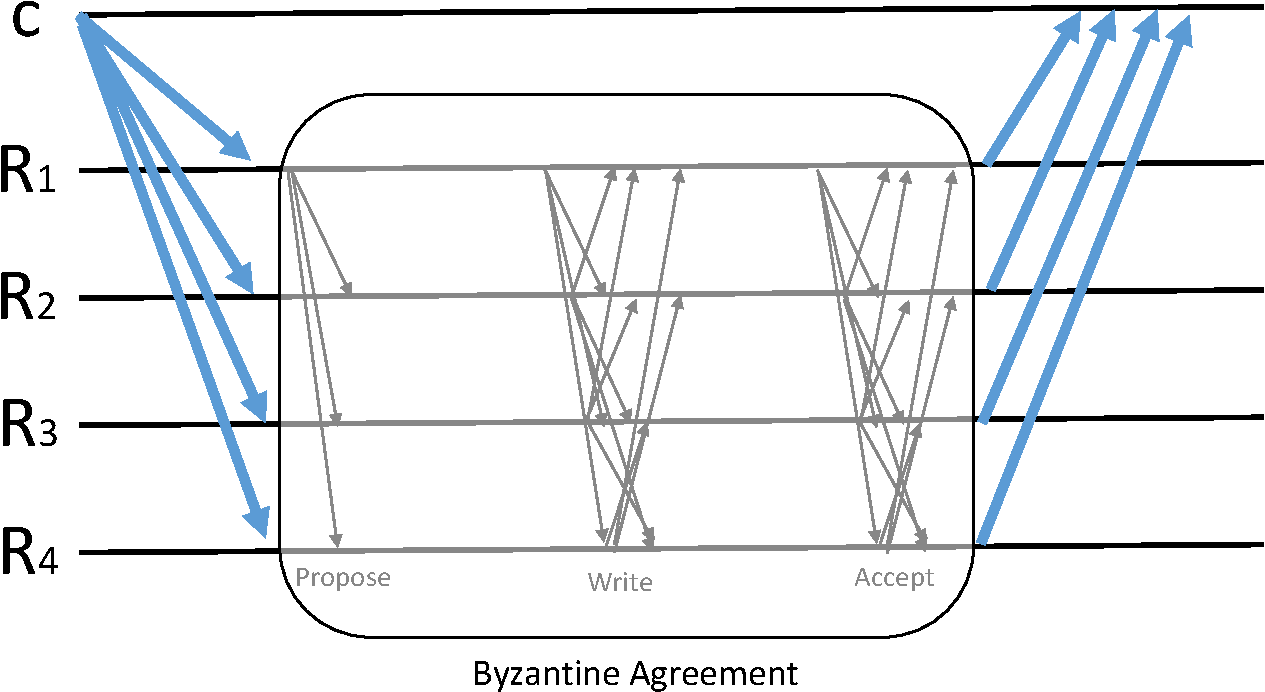
\includegraphics[width=.5\columnwidth]{images/images/bft.pdf}
\caption{Byzantine Fault Tolerance protocol overview.}
\label{fig:bft}
\end{center}
\end{figure}

Although \gls{bft} protocols provide safety to a bound of $f$ faulty nodes, with sufficient time $T$ an adversary eventually compromises $f+1$ nodes.
Then, additional mechanisms are needed to clean the faulty state (e.g., from time to time the nodes are recovered~\cite{Castro:2002}).
However, if a recovered node remains vulnerable to the same attack, the time to compromise $f+1$ becomes smaller as the attacker already knows how to exploit its vulnerabilities.
For this reason, several authors built their models assuming that the nodes fail independently due to some mechanism that provides failure independence (e.g.,~\cite{Castro:2002,Veronese:2013,Sousa:2010}).


\section{Byzantine Fault Tolerance}

Intrusion tolerance was first proposed by Fraga and Powell in 1985~\cite{Fraga:1985} as a solution to address faults without compromising the security of a system. 
Almost 15 years after, \gls{bft} replication became the most common solution to implement intrusion tolerance systems.
Castro and Liskov’s PBFT~\cite{Castro:1999} was the first practical \gls{bft} protocol. 
PBFT implements a \gls{smr} protocol that guarantees both liveness and safety for $\lfloor\frac{n-1}{3}\rfloor$ out of a total of n replicas. 
These properties hold even in asynchronous systems such as the internet. 
PBFT implements a SMR, therefore, it must guarantees that each replica executes the same commands, in the same order, and then it produces the same output. 
The protocol can be briefly described as follows: a client sends a message to all the replicas.
Then, the leader replica has to assign a sequence number to the request and multicast a pre-prepare message to the other replicas. 
If the replicas agree with the leader they send a prepare message to each other. 
At this phase of the protocol, every correct replica agrees on the ordering. 
A commit message is sent by every replica. When a replica receives the commit message from a quorum it executes the message. 
In the end, it replies to the client. 
Every replica shares a key with each other and with clients. These keys are used to authenticate messages with a \gls{mac}. 
The messages that are multicast by the clients are authenticated with a vector of \glspl{mac}. 
Then, each replica verifies its own \gls{mac}.
The authors implemented BFS, a Byzantine fault tolerant Filesystem, to validate this \gls{bft} library. 
The results show that when the workload increases the throughput and latency is nearly the same of a non-replicated system. 
This level of performance encouraged the use of \gls{bft} in common systems, and to develop optimizations to improve \gls{bft} protocols. 
Since the PBFT proposal, some work has been dedicated to improve \gls{bft} protocols (see Table~\ref{tab:bft}):


\begin{table}[!t]
\begin{center}
{\footnotesize
\begin{tabular}{ p{2.5cm}  p{11cm}  }\hline
Zyzzyva~\cite{Kotla:2010}  & Introduces speculation to avoid the expensive three phase commit before processing the requests. This might introduce some inconsistency in the state of the replicas when speculation fails, and the client needs to help replicas to fix the servers’ inconsistency. \\ \hline			
Upright~\cite{Clement:2009} & It provides a straightforward way to also add BFT to crash fault tolerant systems (CFT); \\ \hline	
Aardvark~\cite{Clement:2009b} & Shifts the paradigm to a new design. This design improves the performance under faulty scenarios trading some performance on the normal case; \\ \hline
BFT-SMaRt~\cite{Bessani:2014} & It is modular and multicore-aware. Supports replica reconfiguration and has a flexible programming interface; \\ \hline
COP~\cite{Behl:2015} & It is the most recent BFT implementation that reached 2.4 million operations per second. This was achieved mostly due to BFT architecture changes.\\  \hline  
\end{tabular}
}
\caption{Brief overview of the most relevant BFT works.}
\label{tab:bft}
\end{center}
\end{table}

\paragraph{Summary.} 
Intrusion tolerance has an important role in our work, namely BFT-replication.
We propose a system that enhances intrusion tolerance by adding mechanisms that work on
top of a \gls{bft} replicated system. We need \gls{bft} protocols to guarantee that replicas execute in
the same order and to be able to tolerate some malicious failures in a subset of the replicas.
The implementation of such \gls{bft} protocol is a complex task, particularly if we need to
include mechanisms for state transfer, reconfiguration, and guarantee a good performance.
We prefer to rely on existent libraries than to build a new one.



\section{Replica Rejuvenation}


Software rejuvenation was proposed in the 90's~\cite{Huang:1993,Huang:1995} as a proactive approach to prevent performance degradation and failures due to software aging. 
The first proposals were based on periodical clean-up of the aging effects by restarting some parts of the software. 
This mechanism would postpone failures and restore the performance. 
This solution was implemented using three components: a watchdog process (\texttt{watchd}), a checkpointing library (\texttt{libft}) and a replication mechanism (\texttt{REPL}). 
A primary node executes the application while a backup node has the application inactive. 
The primary also runs the \texttt{watchd} to monitor the application crashes and hangs. 
In the backup, there is another watchdog watching the primary node. 
There is a routine (provided by \texttt{libft}) that periodically makes checkpoints and logging. 
These checkpoints are replicated with REPL in the backup node. 
When the primary node crashes or hangs, it is restarted, and if needed the backup takes his place on the execution.
PBFT-PR~\cite{Castro:2002} and COCA~\cite{Zhou:2002} introduced proactive recoveries in \gls{bft} replicated systems. 
Proactive Recovery is a mechanism that periodically rejuvenates the replicas to clean potential faults or stealth attacks. 
This mechanism allows that an adversary controls some replicas, usually $f$ , during a time window, where the system is vulnerable.
Castro and Liskov presented PBFT-PR~\cite{Castro:2002}, a BFT replication library that does proactive recovery (PR). 
PBFT-PR assumes that replicas will frequently recover. 
Additional assumptions are needed to guarantee the PBFT-PR's liveness and safety during the recoveries: 
(i) Each replica contains a trusted chip to store its private key, and it can sign and decrypt messages without revealing the key; 
(ii) The replicas’ public keys are stored in a BIOS read-only memory, which needs physical access to modify the BIOS; 
And last, (iii) a watchdog timer is used to avoid human interaction to restart replicas. 
The watchdog hands the execution to the recovery monitor, which cannot be interrupted.
Zhou~\etal{} presented COCA~\cite{Zhou:2002}, a fault-tolerant and secure online certification authority that has been built and deployed both in a local area network and on the internet.
COCA uses proactive signature sharing to ensure that when replicas fail and recover there
is no key-leakage. Contrary to PBFT-PR it does not rely on trusted components, but it may
need an administrator to refresh the COCA server keys.
Distler~\etal{} identified virtualization as a useful mechanism to implement proactive recovery in VM-FIT~\cite{Reiser:2007,Distler:2008}. 
The authors assume that an intrusion-tolerant replicated system executes in an untrusted domain, running in \gls{vm}. 
VM-FIT executes in a trusted domain, i.e., the \gls{vmm}. 
Virtualization allows the isolation between the untrusted and the trusted domains. 
Therefore, it can trigger recoveries from the trusted domain in a synchronous manner. 
Moreover, virtualization reduces downtime of the service during the recovery and makes the state transfer between replicas more efficient. 
The authors implemented this system using the Xen hypervisor to get the two domains: the trusted domain is the Xen Dom0, and the replicas run in the untrusted domains, DomUs.

Sousa~\etal{} improved the state-of-the-art recovery algorithms by introducing \gls{prrw}~\cite{Sousa:2010}. 
This technique removes the effects of faults ``immediately''. 
\gls{prrw} accelerates the rejuvenation process by detecting the faulty replicas behavior and forcing them to recover without sacrificing periodic rejuvenations. 
This type of technique can only be implemented with synchrony assumptions as the recoveries are time triggered~\cite{Sousa:2005}. 
To address this need the authors proposed an hybrid system model: the payload is an any-synchrony subsystem, and the wormhole is a synchronous subsystem. 
The authors implemented this system using the Xen hypervisor as the wormhole. 
Zhao~\etal{}~\cite{Zhao:2010} improved~\cite{Sousa:2010} with an algorithm to schedule the rejuvenations that is adaptable to a constant monitoring of the network and CPU/memory performance.

\paragraph{Summary.} \gls{bft} replication with proactive recovery represents one of the cornerstones of intrusion tolerance. 
PR allows the system to reduce the vulnerability window of the replicated system drastically. 
BFT replication with PR guarantees the system's correctness while the replicas recover faster than $f+1$ replicas become faulty. 
One limitation of PR is that there must be a trusted element somewhere to implement this mechanism. 
Some works use hardware timers while others resort to virtualization to separate the execution domains. 
In our proposal, we will adopt an architecture similar to~\cite{Distler:2008} and ~\cite{Sousa:2010}. 
However, our solution will implement a different (from~\cite{Sousa:2010}) algorithm to proactively trigger recoveries.


\section{Diversity}

In some of the works presented before, the correctness is ensured under the assumption that replicas fail independently. 
Often the authors assume that fault independence is achieved using diversity~\cite{Castro:2002,Sousa:2010}. 
Diversity can be implemented in different ways~\cite{Deswarte:1999,Obelheiro:2006}, which may differ in the mean and the amount of diversity generated, but the goal is the same: to create different attack surfaces. 
The goal is to make the discovery of common vulnerabilities more difficult. 
We present at least three different ways to generate diversity: 
(i) N-version programming consists in design/implementation of different program binaries (from the same or different source code); 
(ii) Randomization implements different memory schemes; 
and (iii) Off-the-shelf diversity comprises the use of different products with the same functionality but taking advantage of implementations that are already available.


\paragraph{N-version programming}
N-version programming is a technique used to create diverse software components~\cite{Avizienis:1977,Knight:1986,Chen:1995}.
The main idea behind this mechanism is to develop N different implementations of the same specification. 
These implementations can be implemented by N different developers or using translators to N different programming languages.

\paragraph{Artificial diversity.} 
Forrest~\cite{Forrest:1997} suggested randomized program transformations to introduce application diversity. 
They have made modifications on the gcc, a C compiler, in such a way that during the compiling time gcc inserts random padding
into each stack frame. 
Linger presented stochastic diversification tool to swap code structures~\cite{Bairavasundaram:2009,Larsen:2014}. 
The diverse versions are generated during the source code compilation. 
The main idea of these works is to make the intruder’s work more difficult when exploiting buffer overflow vulnerabilities.
Bhatkar~\etal{}~\cite{Bhatkar:2003} proposed a solution based on memory address obfuscation (i.e., \gls{aslr}). 
Their solution transforms object files and executables at the link-time and load-time, without kernel or compiler modifications. 
The goal is to ensure that an attack that succeeds in one target will not succeed on the other targets. 
Each time the program is executed its virtual addresses and data are randomized, and therefore the attacker needs to find new ways to exploit memory errors, like buffer overflows. 
However, a recent work proved that solutions like ASLR are vulnerable to attacks~\cite{Bittau:2014}.
A few works propose the usage of compilers that generate different executables~\cite{Platania:2014,Roeder:2010,King:2016}.


\paragraph{Off-the-shelf diversity.}
The two previous solutions generate diversity before the software’s distribution. 
\gls{ots} diversity does not need pre-distribution of diverse mechanisms. 
It relies on the existence of different software components that are ready to be used.
There are plenty of different free products that provide the same functionality and were developed by different vendors. 
In other words, \gls{cots} diversity is like an opportunistic N-version programming.
Totel~\etal{} proposed an \gls{ids} based on design diversity~\cite{Totel:2005}.
The authors described an architecture that uses a set of replicated \gls{cots} servers, a proxy, and an \gls{ids}. 
The proxy is responsible for forwarding the requests from the client to every \gls{cots} server. 
When the servers reply, the proxy sends the responses to the \gls{ids} to be analyzed. 
The IDS compares the responses from the \gls{cots} servers and if it detects some differences an alarm is raised. 
Then the proxy votes the responses and replies to the clients. 
The authors developed an algorithm to detect intrusions and tested their solutions against Snort~\cite{snort} and WebStat~\cite{Vigna:2003}. 
The results show that using diverse-\gls{cots} service (e.g., http) allows the \gls{ids} to deliver fewer alarms without missing the intrusions.
Gashi~\etal{} made an experimental evaluation of the benefits of adopting diversity of SQL database servers~\cite{Gashi:2007}. 
The authors analyzed bug reports of four database servers (Post-greSQL, Interbase, Oracle, and Microsoft SQL Server) and verified which products were affected by each bug reported. 
They have found few cases of a single bug affecting more than one server. 
In fact, there were no coincident failures in more than two of the servers.
The conclusion is that \gls{ots} database servers’ diversity is an effective mean to improve system's reliability. 
However, the authors recognize the need for SQL translators, to increase the interoperability between servers in the replicated scenario.
Han~\etal{}. made a systematic analysis of the effectiveness of using \gls{ots} diversity to improve system's security~\cite{Han:2009}. 
First, the authors found if there were \gls{ots} software substitutes to provide the same functionality. 
Then, they determined if the \gls{ots} software shared the same vulnerabilities.
And if so, if the same vulnerability could be exploited with the same attack. 
In this study, more than 6k 1 vulnerabilities were analyzed, which were published in the \gls{nvd} on the year 2007. 
The results showed that 98.5$\%$ of the vulnerable software have substitutes. 
Moreover, the majority of them either did not had the same vulnerabilities or could not be compromised with the same exploit code. 
It is not expected that a single exploit works in different \glspl{os} because each one has a different memory scheme and different filesystems. 
Even between versions from the same \gls{os}, the low-level functions change across the versions. 
The study also concluded that 22.5$\%$ of the vulnerabilities were present in multiple software. 
However, only 7.1$\%$ from those vulnerabilities were present in software that offers the same service. 
The study findings are a good sign that diversity can improve a system’s dependability.
In a previous work, we studied \gls{ots} OSes diversity~\cite{Garcia:2014}. 
Similar to \cite{Han:2009} this study was carried out taking vulnerability feeds from \gls{nvd}. 
However, our work was only focused on OSes, and the data collected comprised 11-year of vulnerability reports. 
Our goal was to find to what extent different OSes shared common vulnerabilities. 
In this study, we analyzed 2270 vulnerabilities entries manually, where they were classified in different categories. 
Then, we defined three types of servers: (i) a server that contains most the packages/applications available (Fat server); (ii) a server that does not contain unnecessary applications to a certain
service (Thin server); and (iii) a thin server but with physically controlled access (Isolated hin server). 
We assumed that the third setting it is the most advisable for critical systems, since additional care is taken to install and setup its configuration. 
For each configuration, we compared all the common vulnerabilities in pairs of OSes. 
As expected, in the Isolated thin server, the number of common vulnerabilities was considerable less than in the other configurations. 
There was only 1 vulnerability that was shared among six OSes, 2 that were shared among five OSes, and 130 that are shared between two OSes. 
We went further in the study and looked for common vulnerabilities in different versions of the same OS. 
We have found evidence that suggests that using OS diversity in a replicated system can improve its dependability. 
Even if few OSes are employed, it is possible to achieve vulnerability independence just with different versions.



Larsen~\etal{} made a study with several examples on how to apply diversity~\cite{Larsen:2014,Larsen:2015}. 
The paper explains in detail what to diversify, from single instructions to an entire program. 
They also explain the three types of security impacts when diversity is applied: entropy analysis, attack-specific code analysis, and logical argument. 
However, they also point that there is no consensus on how to evaluate the efficacy of diversity. 



\paragraph{Summary.}
We presented three different techniques that support diversity as a fault-tolerant mechanism. 
N-version programming is the most costly, since it needs different developers or additional programs to verify if the automatic translation works. 
On the contrary, \gls{ots} and randomization diversity are almost for free. 
The first one can be obtained from free sources that are ready to be used, and the second one is automatic and already supported
in most OSes. 
Diversity still has some gaps that must be addressed to make it an effective building block of intrusion tolerance. 
For example, how to measure diversity in such a way that failure independence can be guaranteed?



\section{Risk Management}

Jumratjaroenvanit and Teng-amnuay~\cite{Jumratjaroenvanit:2008} described vulnerability life-cycles presenting their different stages. 
The authors goal was to understand how different dates can be useful to estimate the probability of an attack. 
The authors methodology was to collect and analyze data on the discovery, disclosure, and exploit dates, exploit and patch availability, all from public data sources. 
They used this information to define five life cycle types: (i) \gls{zda}, which typically is a done by a black-hat and is defined by the date of disclosure and exploit being the same; (ii) \gls{pzda}, is a \gls{zda} but with a patch already available, but not applied; 
(iii) \gls{ppzda}, is a \gls{pzda} but does not matter if the patch is available or not; 
(iv) \gls{poa}, it is a zero-day vulnerability. 
The most influential variables were the code that was scrutinized by a the tester with access to the source code, and the code that was analyzed with some static tool before. 
On the contrary, results showed that language safety was the less influent factor. 
The main result of the study was that two weeks of work were enough to have a 50\% chance of finding a zero-day vulnerability. 
Sometimes, 53 hours were enough to find one vulnerability with more than 95\% of probability.


Okhravi~\etal{} presented TALENT a framework for live migration of critical infrastructures across heterogeneous platforms~\cite{Okhravi:2014,Okhravi:2009}. 
The idea was to create a moving target that difficult the success of advanced targeted attacks. 
TALENT implements OS level virtualization with containers, which allows the system to migrate the OS between machines periodically or upon detection of malicious activity. 
The virtualization was implemented with OpenVZ and LXC for Linux, Virtuozzo for Windows, and Jail for FreeBSD. 
The network was also virtualized, more precisely, a second layer of virtualization was used to migrate the IP address from one container to another. 
Even an established ssh session was preserved during the migration. 
Additionally, the state of the application also had to be migrated by employing a checkpointing technique. 
When all the programs were checkpointed, the state was saved and then was migrated by mirroring the filesystem. 
The filesystem synchronization took 98.7\% of the migration time. 
The authors decided to focus on optimizing the filesystem synchronization. 
In the optimized version, the filesystem synchronizes in periodic intervals by sending the differences to the destination. 
Therefore, the migration was made seamless to the application. 
TALENT also had a risk assessment, called operation assessment, which monitored and adjusted the diverse components using vulnerability information. 
However, there was almost no details on how the risk was measured and on how to adapt to the threats in an efficient manner.

Guo and Bhattacharya addressed the problem of \gls{bft} replicas fault independence~\cite{Guo:2014}.
The authors proposed different replicas configurations using OTS OSes to increase the diversity among the replicas. 
There was a set of different configurations that could build a replicated system. 
Each configuration was composed of different \gls{os}. 
The authors proposed a formalization of the virtual replica diversification problem. 
They used a game-theory approach to find an optimal diversification strategy for the defender's side. 
The authors validated their model with the \gls{nvd} data used in~\cite{Garcia:2012}.
Wang~\etal{} proposed a different approach to measure the risk~\cite{Wang:2014}. 
The study explored how many zero-day vulnerabilities were required to compromise a network. 
They assumed that zero-day vulnerabilities typically do not occur at the same time, however the solution did not depend on any statistical model. 
The reasoning behind the proposal was novel, e.g., on the method to find the complexity of multiple zero-day vulnerabilities in a N-node network.

Newell~\etal{} ~\cite{Newell:2015} presented a solution to assign diversity variants among network nodes to increase the network's resiliency.

Sabote~\etal{}~\cite{Sabottke:2015} presented a study that used non-common vulnerability data sources, i.e., Twitter data (e.g., specific words, the number of retweets, and replies, information about
the users posting these messages), to find exploit data. 
The authors made a quantitative and qualitative exploration of the vulnerability-related information disseminated on Twitter.
They developed a Twitter-based exploit detector to provide an adequate response in a such short time frame. 
This allows the security community to foresee the exploit activity before the information reaches the de facto disclosure data sources like \gls{nvd} and ExploitDB.
However, to complement and strength their information results they also used sources like \gls{nvd}, \gls{osvdb}, Exploit-DB, Microsoft Security Advisories and Symantec WINE. 
The authors distinguished the real-world exploits from the proof-of-concept exploits, as the latter are by products of the disclosure process. 
The real-world exploits typically are not known until a critical zero-day attack occurs. 
The authors used \gls{svm} to classify exploits in the social media and tested how robust it was to attacks, i.e., if a powerful attack could manipulate the information on Twitter with a false account and false data. 
The results showed that with their proposal they could be confident with the predictions. 
For example, the \gls{svm} classifier set to a precision of 25\% could detect the Heartbleed exploits within 10 minutes of its first appearance on Twitter. 
They also showed that organizations like \gls{nvd} overestimate the severity of some vulnerabilities that never become in fact exploited.
However, their work did not focus on the discovery of the zero-day vulnerabilities, which is relevant for our research.

\paragraph{Summary.} We presented several works that carry out for risk assessment in a way to prevent exploits or to take action upon vulnerability detection. 
This is the last building block that intrusion tolerance is missing. 
There is a lot of relevant free information available to address the security and dependability of software. 
In a replicated context this information is even more relevant. 
First, to react upon vulnerability/exploit disclosures, and second to select what configurations are less vulnerable to common weakness. 
We want to explore the free available data to improve, the dependability and security of intrusion-tolerant systems, by ensuring the assumption of failure independence with evidence supported by  relevant data.



\section{Pratical BFT System with Diversity}


In the last two decades there were a number of \gls{bft} protocols and systems deemed ``practical'' (e.g.,~\cite{Castro:2002,Kotla:2010,Veronese:2013,Aublin:2015,Behl:2015,Behl:2017,Liu:2016,Yin:2003}).
Most of these systems either ignore the issue of fault independence or simply assume it is solved in some way (e.g., N-version programming~\cite{Chen:1995} or \gls{ots} diversity~\cite{Gashi:2007,Garcia:2014}).
In principle, \system can support the execution of all these systems/protocols, as long as they support, or are extended to support, replica group reconfigurations, just like BFT-SMaRt~\cite{Bessani:2014}.
In this section, we discuss the few previous works that address the issue of diversity in \gls{bft} systems. 

BASE~\cite{Rodrigues:2001} is an extension of PBFT~\cite{Castro:1999} that explores opportunistic \gls{ots} diversity in \gls{bft} replication. 
The system provides an abstraction layer for running diverse service codebases on top of the PBFT library.
The key issue addressed by BASE is how to deal with different representations of the replica's state, allowing a replica that recovers from a failure to rebuild its state from other replicas. 
BASE was evaluated considering four different OSes and their native \gls{nfs} implementations: Linux, OpenBSD, Solaris, and FreeBSD.
The results, from 16 years ago, show the same trends we observed: performance varies significantly when diversity is considered.
Differently from \system, BASE does not address the selection of replicas or the reconfiguration of a replica group.

In order to support long-running services, Castro and Liskov~\cite{Castro:2002} introduced the notion of proactive recovery for \gls{bft} services. 
The objective is to rejuvenate replicas periodically to remove stealth attackers and support the execution of long-running services. 
All works on \emph{safe} proactive recovery consider the use of trusted local component on each replica to trigger the periodic recoveries~\cite{Castro:2002,Sousa:2010,Roeder:2010,Platania:2014,Distler:2011}.
%, and some of them even support reactive recoveries to deal with service degradations caused by detectable attacks~\cite{sousa:pc}.
A common weakness of most of these works is that they do not support diversity, therefore a compromised replica can be attacked immediately after its recovery by exploiting the same vulnerability.
The two noticeable exceptions are discussed in the following.

Roeder and Schneider~\cite{Roeder:2010} propose an intrusion tolerance technique called \gls{po} for supporting a different type of diversity from \system.
The idea is, instead of changing \glspl{os} or other off-the-shelf component of the replica, \gls{po} changes the application and library code periodically preserving the original semantics using program transformations, i.e., system call obfuscation reordering, memory randomization, and functions return checks (through an IBM \textit{gcc} patch that inserts and checks a random value after the functions return).
Each replica generates its own obfuscated executable from a read-only device containing the ``master code'' based on time-triggered epochs that a controller triggers in a secure way through a trusted component similar to \system' \gls{ltu}.
All obfuscation mechanisms were implemented and evaluated on OpenBSD 4.0, and their results show that PO adds a little extra overhead to the non-\gls{po} execution.

Similarly to \gls{po}, Platania~\etal{}~\cite{Platania:2014} proposed a compiler-based diversity for the Prime \gls{bft} protocol~\cite{Amir:2011} using the MultiCompiler tool~\cite{Homescu:2013}. 
This compiler creates diverse binaries from the same source code through randomization and padding techniques.
The authors also proposed a theoretical rejuvenation model that receives as input: the probability of a replica being correct over a year ($c$); the number of rejuvenations per day across the whole system ($r$); the number of replicas ($n$); and the system's lifetime. 
Although operators can control only $r$ and $n$, the authors suggest (but does not show how) that $c$ can be estimated using \gls{osint} from the internet (CERT alerts, bug reports, and other historical data).
The authors implemented their solution in two settings, including a virtualized environment provided by the Xen Hypervisor.
In this setting, each replica executes in a Linux \gls{vm}, the recovery watchdog runs in a trusted domain of the same machine, and the proactive-recovery controller runs in another physical machine, in an architecture similar to ours.


\paragraph{Summary.} 
Diversity is becoming one of the building blocks of intrusion tolerance, alongside with \gls{bft} and rejuvenations. 
We presented few works that already used somehow diversity in intrusion-tolerant systems. Some of the works employed opportunistic \gls{ots} components to create diversity among the replicas. 
We do not discard the possibility of using other diversity techniques, such as randomization. 
However, in our work we are interested in \gls{ots} diversity because it is possible to estimate the vulnerability of each component. 
These works are still limited to that extent, i.e., there are none or few concerns on how to create diversity to avoid common failures. 
Most of the works implement diversity assuming complete fault independence, but that is unrealistic. 
For example, different \gls{ots} \glspl{os} can share the same weaknesses due to some shared libraries or kernel code. 
There is a need to understand how diversity can be efficiently employed in a replicated system to make the failure independence sound. 
Moreover, further work is still necessary to create automatic mechanisms that abstract diversity management for the administrators.

Both \gls{po} and the work from Platania~\etal{} improve the diversity of applications and replication libraries,\footnote{It should be noted, however, that recent studies have been shown that the benefits of these techniques are limited~\cite{Snow:2013,Bittau:2014}.} but not on \glspl{os} and other \gls{ots} components used by replicas.
Therefore, \system complements these services, as well as any proactive recovery system,\footnote{In particular, the ones that support proactive and reactive recoveries~\cite{Sousa:2010}.} by assessing and monitoring the potential risk of common-mode failures in a replicated service, and selecting appropriate replacements as the threat landscape evolves.

\system exploits the opportunistic \gls{ots} diversity derived from the existence of many version for \glspl{os}, \glspl{db}, Web Servers, \gls{jvm}, etc.
Several studies show that different versions of these components significantly increase chances of avoiding common-mode failures~\cite{Gashi:2007,Garcia:2014,Gorbenko:2011}.
Although we focus only on OSes in our \system prototype, the same techniques can be used to evaluate and deploy full diverse software stacks in the replicas.


\section{Final Remarks}






